\section{Graph embeddings}
\subsection{}

\begin{frame}{\alert{Text}: sparse symbolic representation}

\begin{center}
	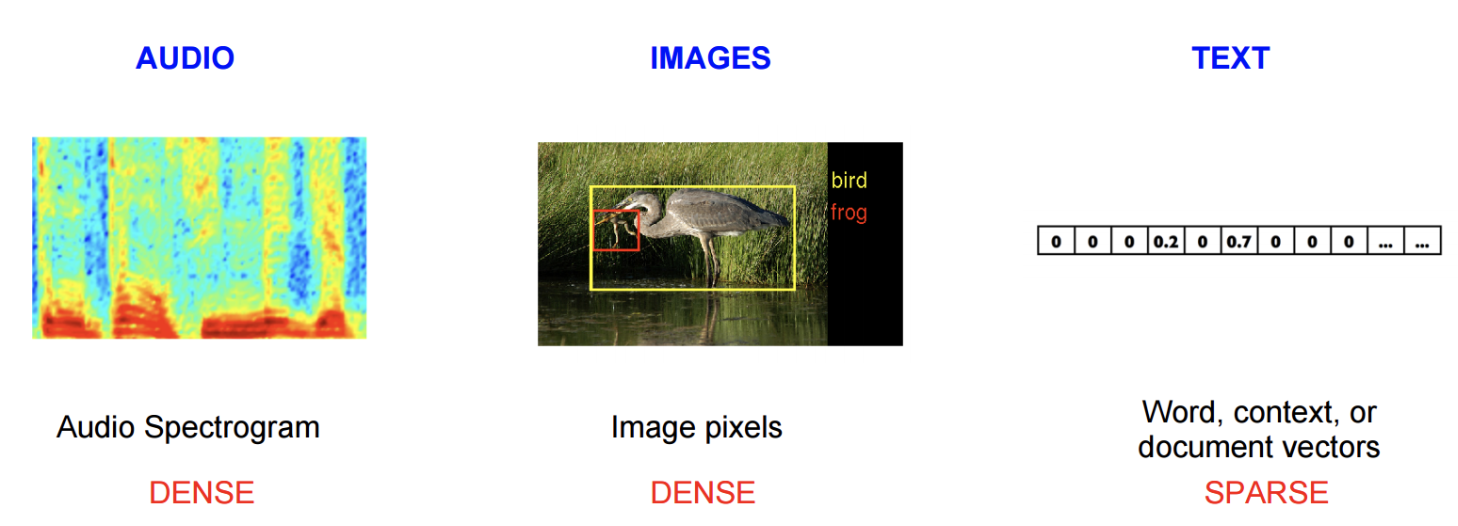
\includegraphics[width=\textwidth]{figures/w2v}
\end{center}

\pause 

Image source: \url{https://www.tensorflow.org/tutorials/word2vec}
	
\end{frame}




\begin{frame}{\alert{Graph}: sparse symbolic representation}

\begin{center}
	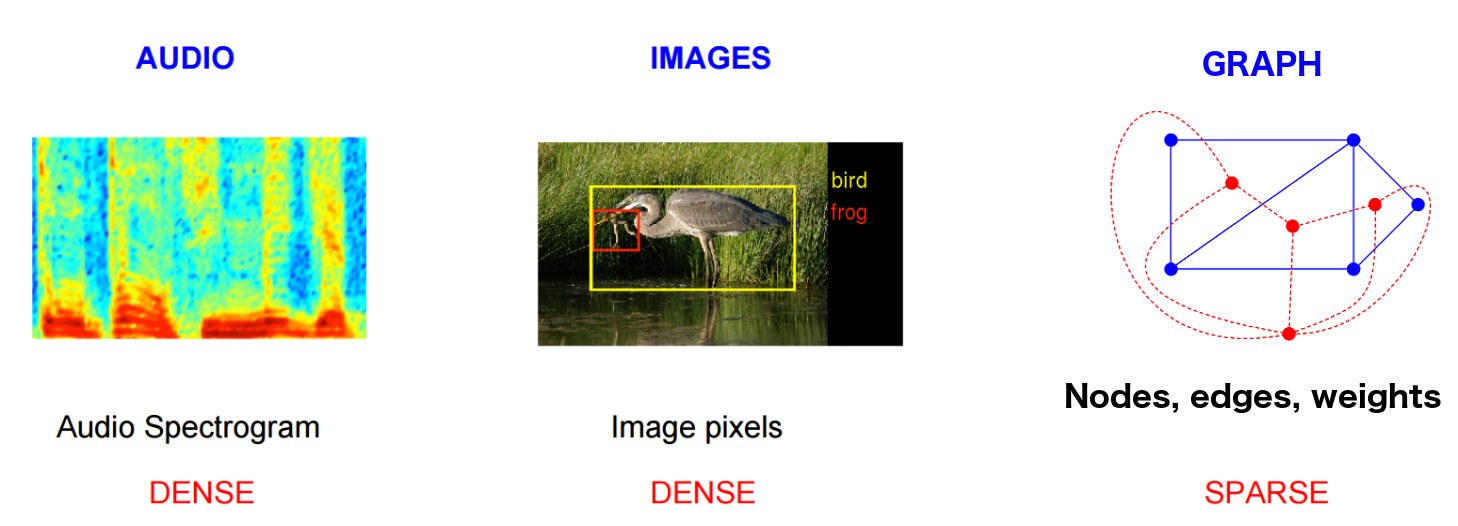
\includegraphics[width=\textwidth]{figures/g2v}
\end{center}
	
\end{frame}


\begin{frame}{Embedding graph into a vector space}

From a \textbf{survey on graph embeddings}~\cite{hamilton2017representation}:

\begin{center}
	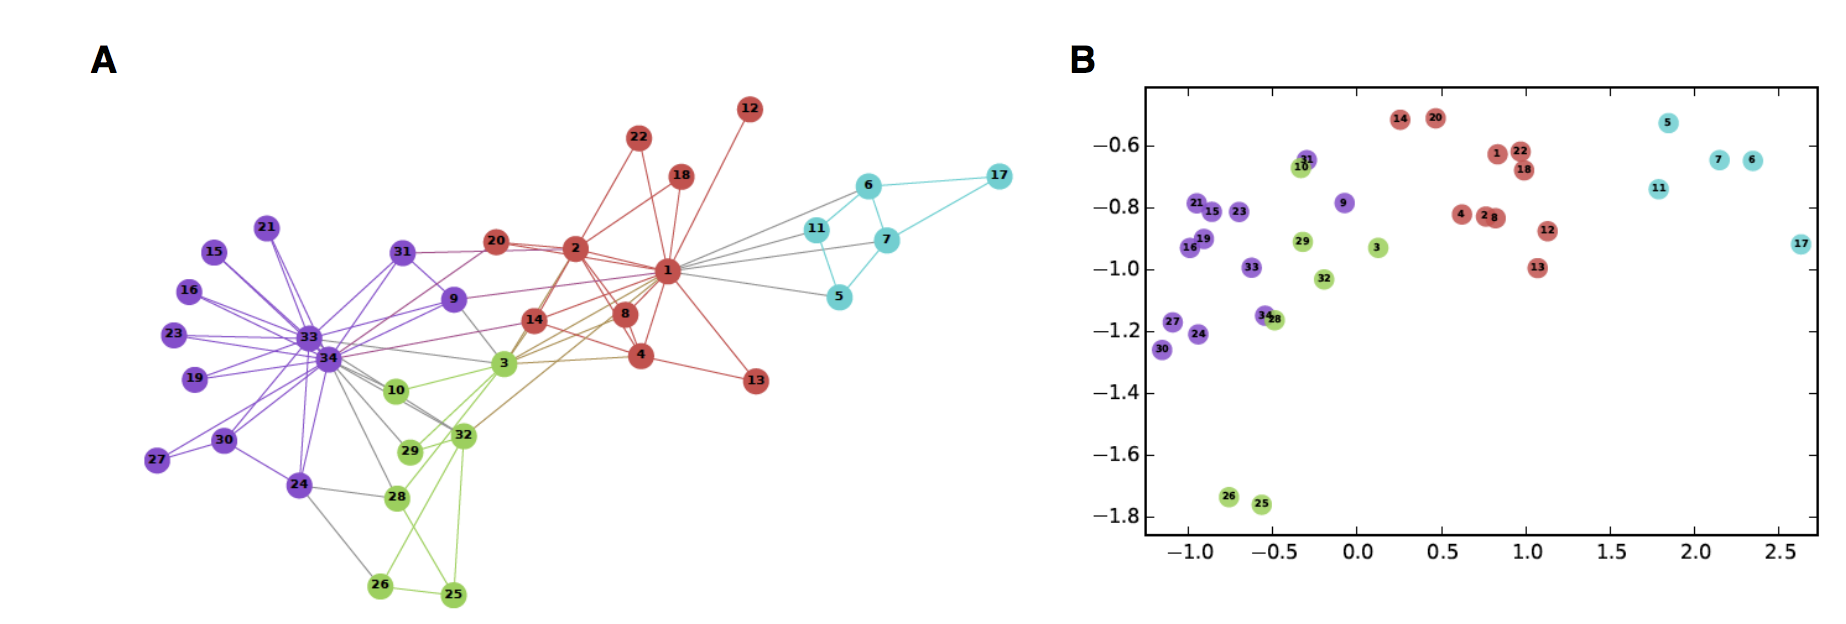
\includegraphics[width=\textwidth]{figures/ge-fig1}
\end{center}

	
\end{frame}



\begin{frame}{Learning with an ``autoencoder''}

From a \textbf{survey on graph embeddings}~\cite{hamilton2017representation}:

\begin{center}
	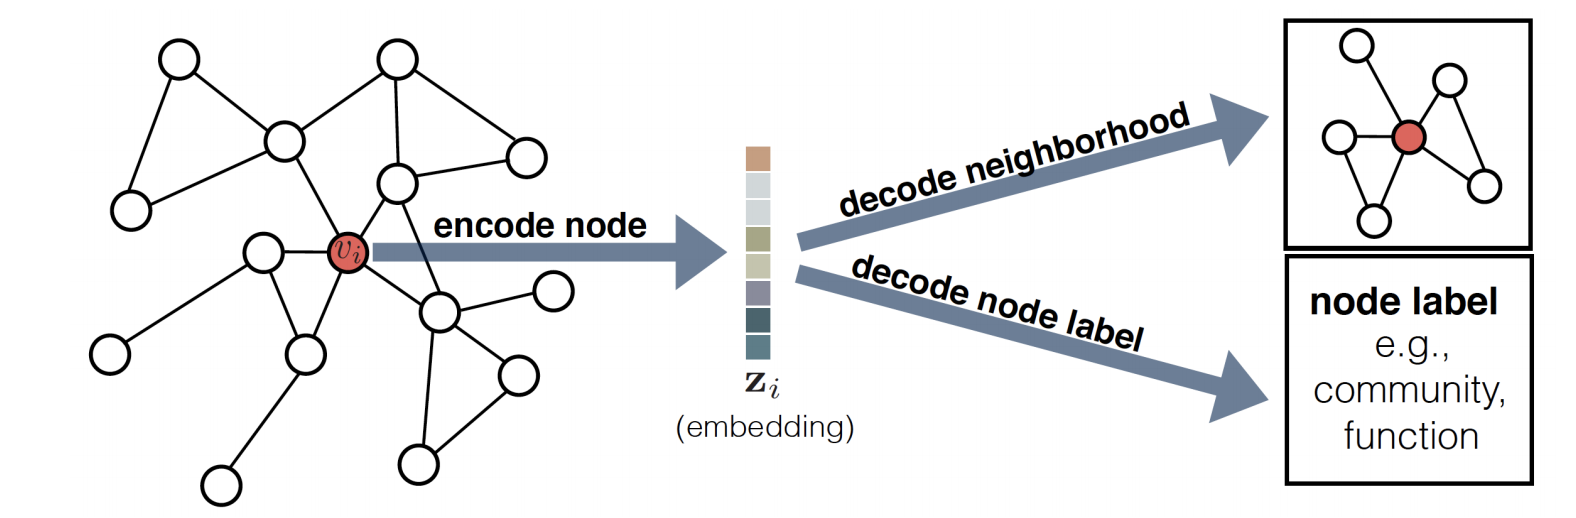
\includegraphics[width=\textwidth]{figures/ge-fig2}
\end{center}

	
\end{frame}




\begin{frame}{Some established approaches}

From a \textbf{survey on graph embeddings}~\cite{hamilton2017representation}:

\begin{center}
	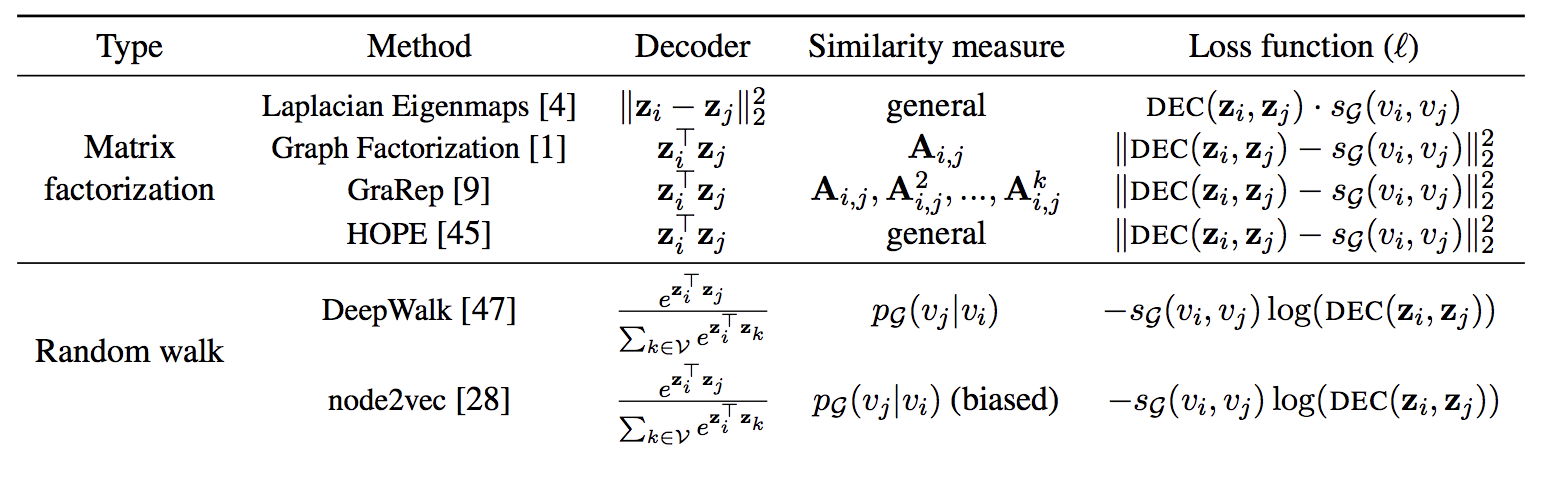
\includegraphics[width=\textwidth]{figures/ge-fig3}
\end{center}

	
\end{frame}
